\documentclass[border=0pt]{standalone}
\usepackage{graphicx}
\usepackage{tikz}
\usepackage{helvet}
\renewcommand{\familydefault}{\sfdefault}
\usetikzlibrary{calc}
\definecolor{ba}{HTML}{505ED5}
\definecolor{argos}{HTML}{D74D3D}
\definecolor{sindy}{HTML}{8EB63D}
\newcommand{\Tag}[1]{{\fontsize{8}{9}\selectfont\bfseries #1}}
\newcommand{\Lab}[1]{{\fontsize{7}{8}\selectfont #1}}
\begin{document}
\begin{tikzpicture}[x=1mm,y=-1mm]
\node[anchor=north west, inner sep=0pt] at (0.000,0.000) {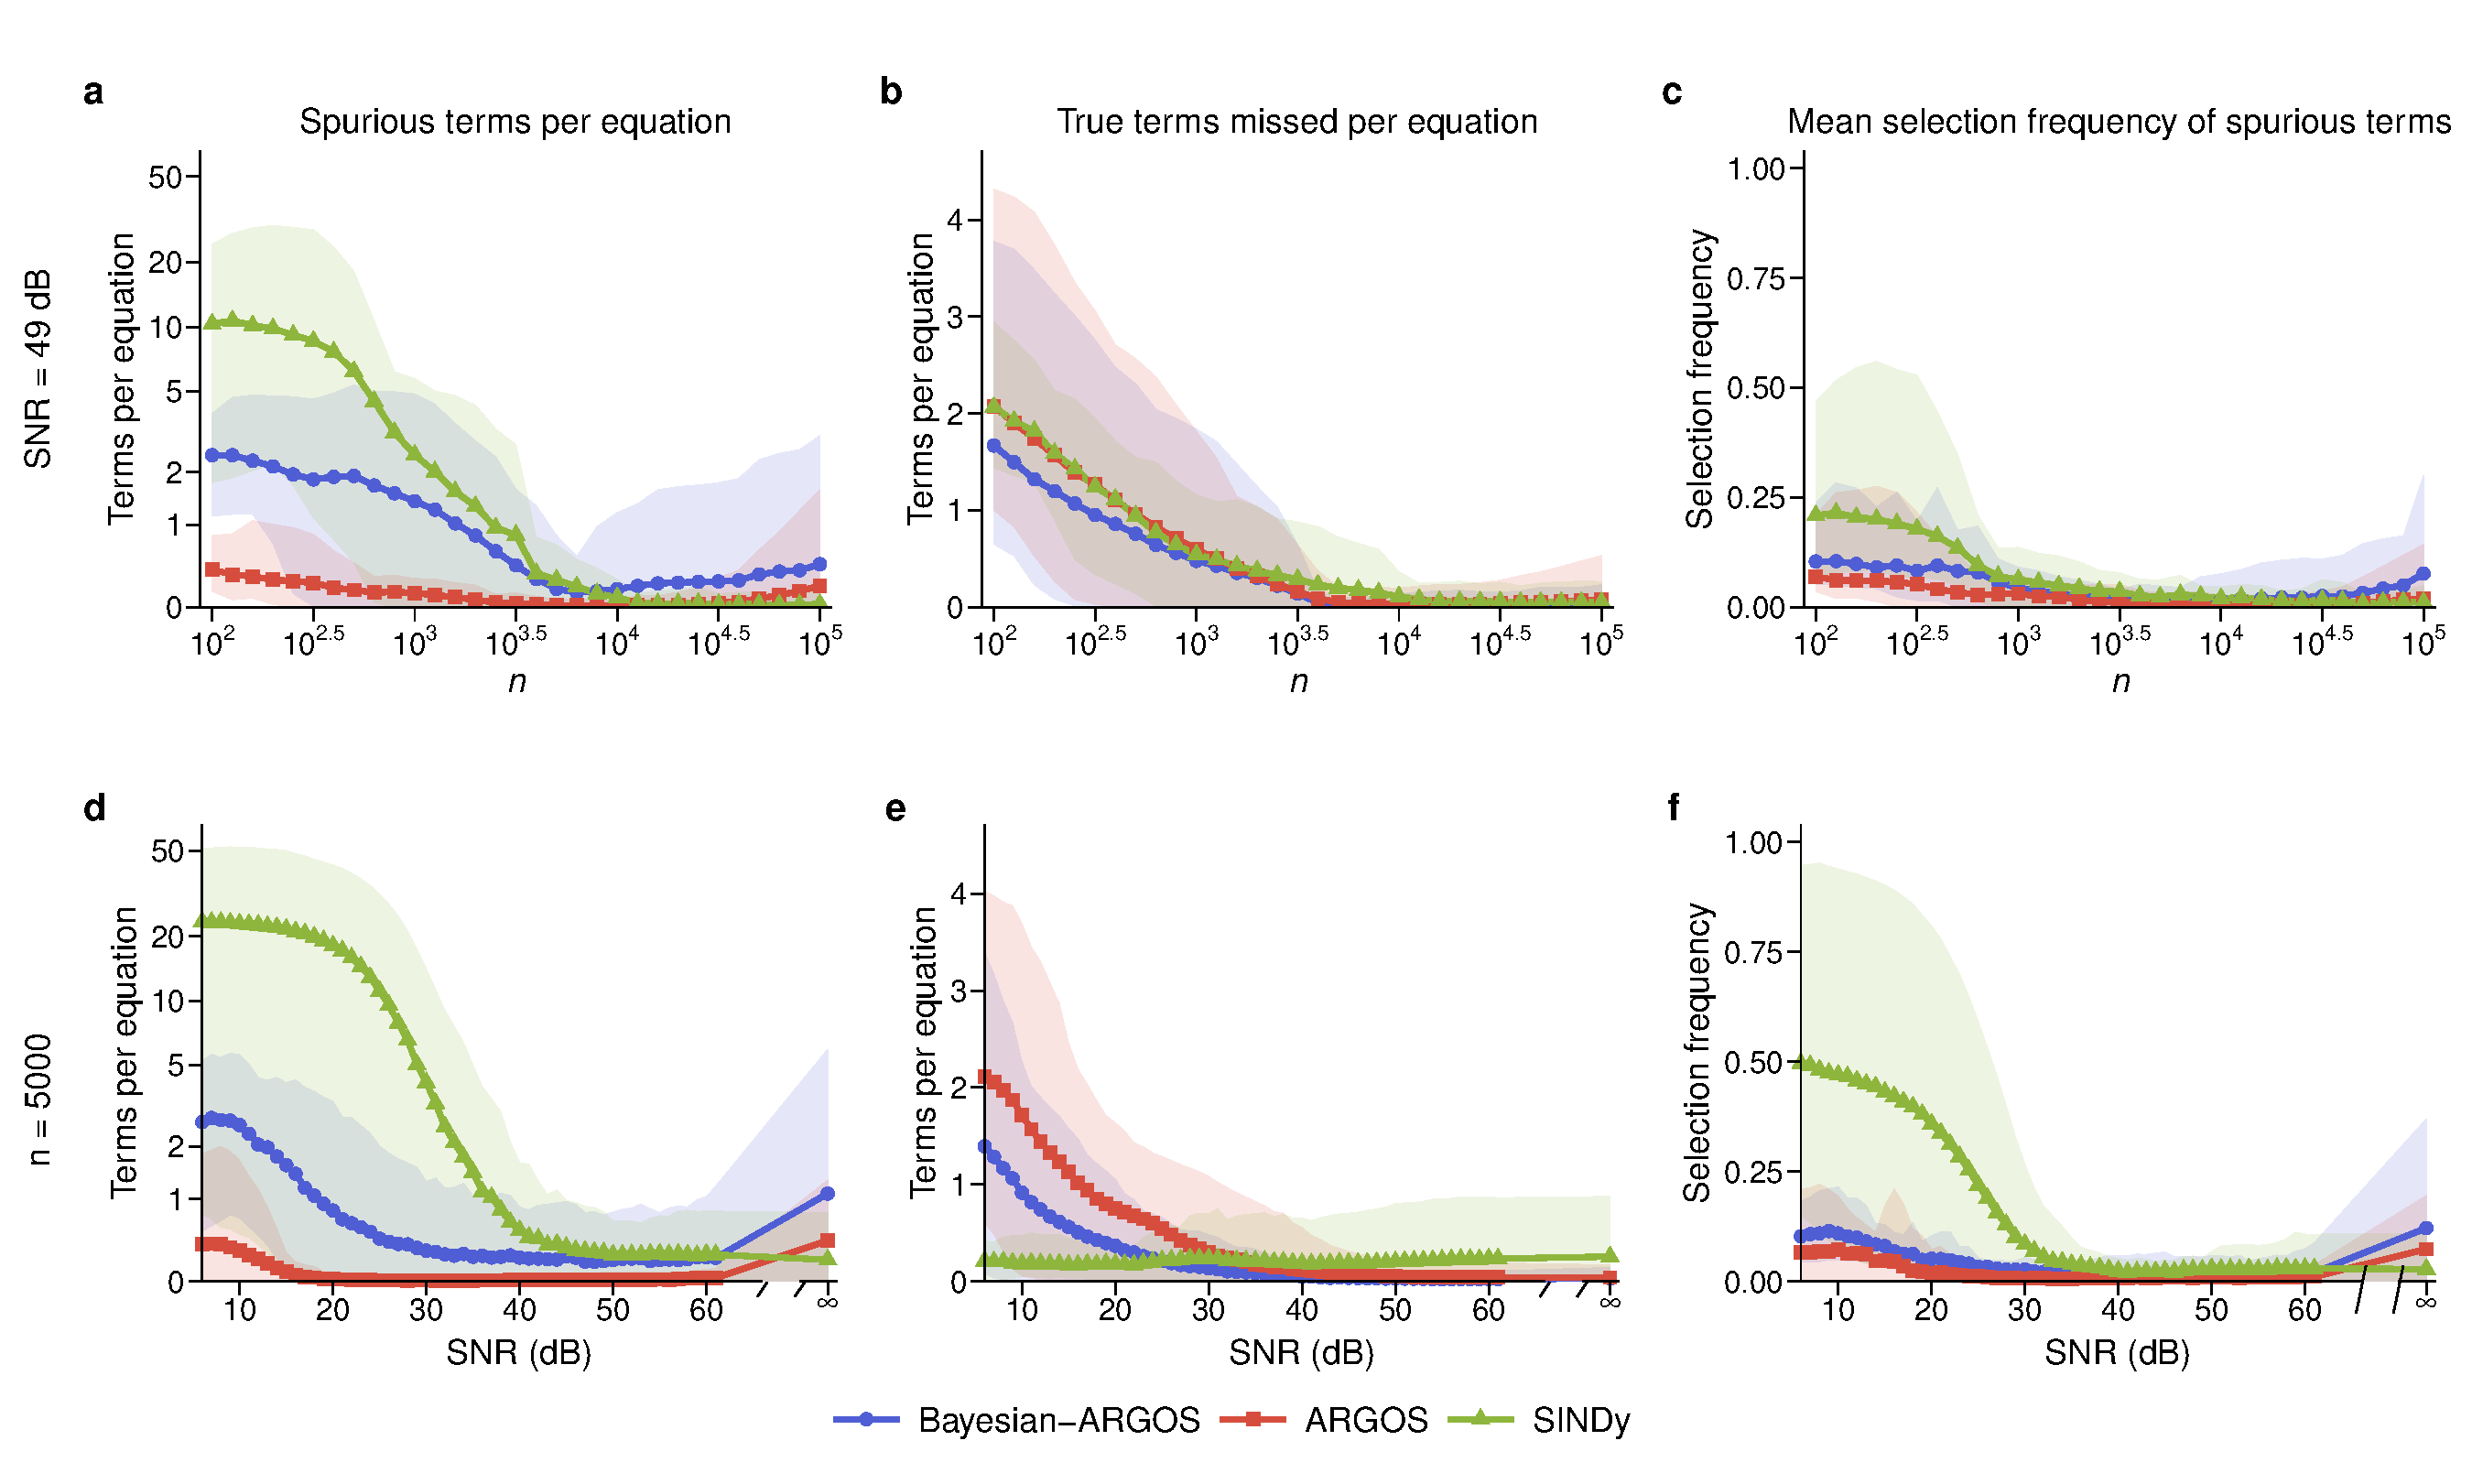
\includegraphics[width=183.000mm]{fig6_block_a.pdf}};
\node[anchor=north, inner sep=0pt] at (91.500,111.356) {\Lab{Lorenz, SNR = 49 dB, 100 trials per ring}};
\node[anchor=north west, inner sep=0pt] at (0.000,115.456) {\Tag{g}};
\node[anchor=north, inner sep=0pt] at (29.500,115.856) {\Lab{Bayesian-ARGOS}};
\node[anchor=north west, inner sep=0pt] at (0.000,119.456) {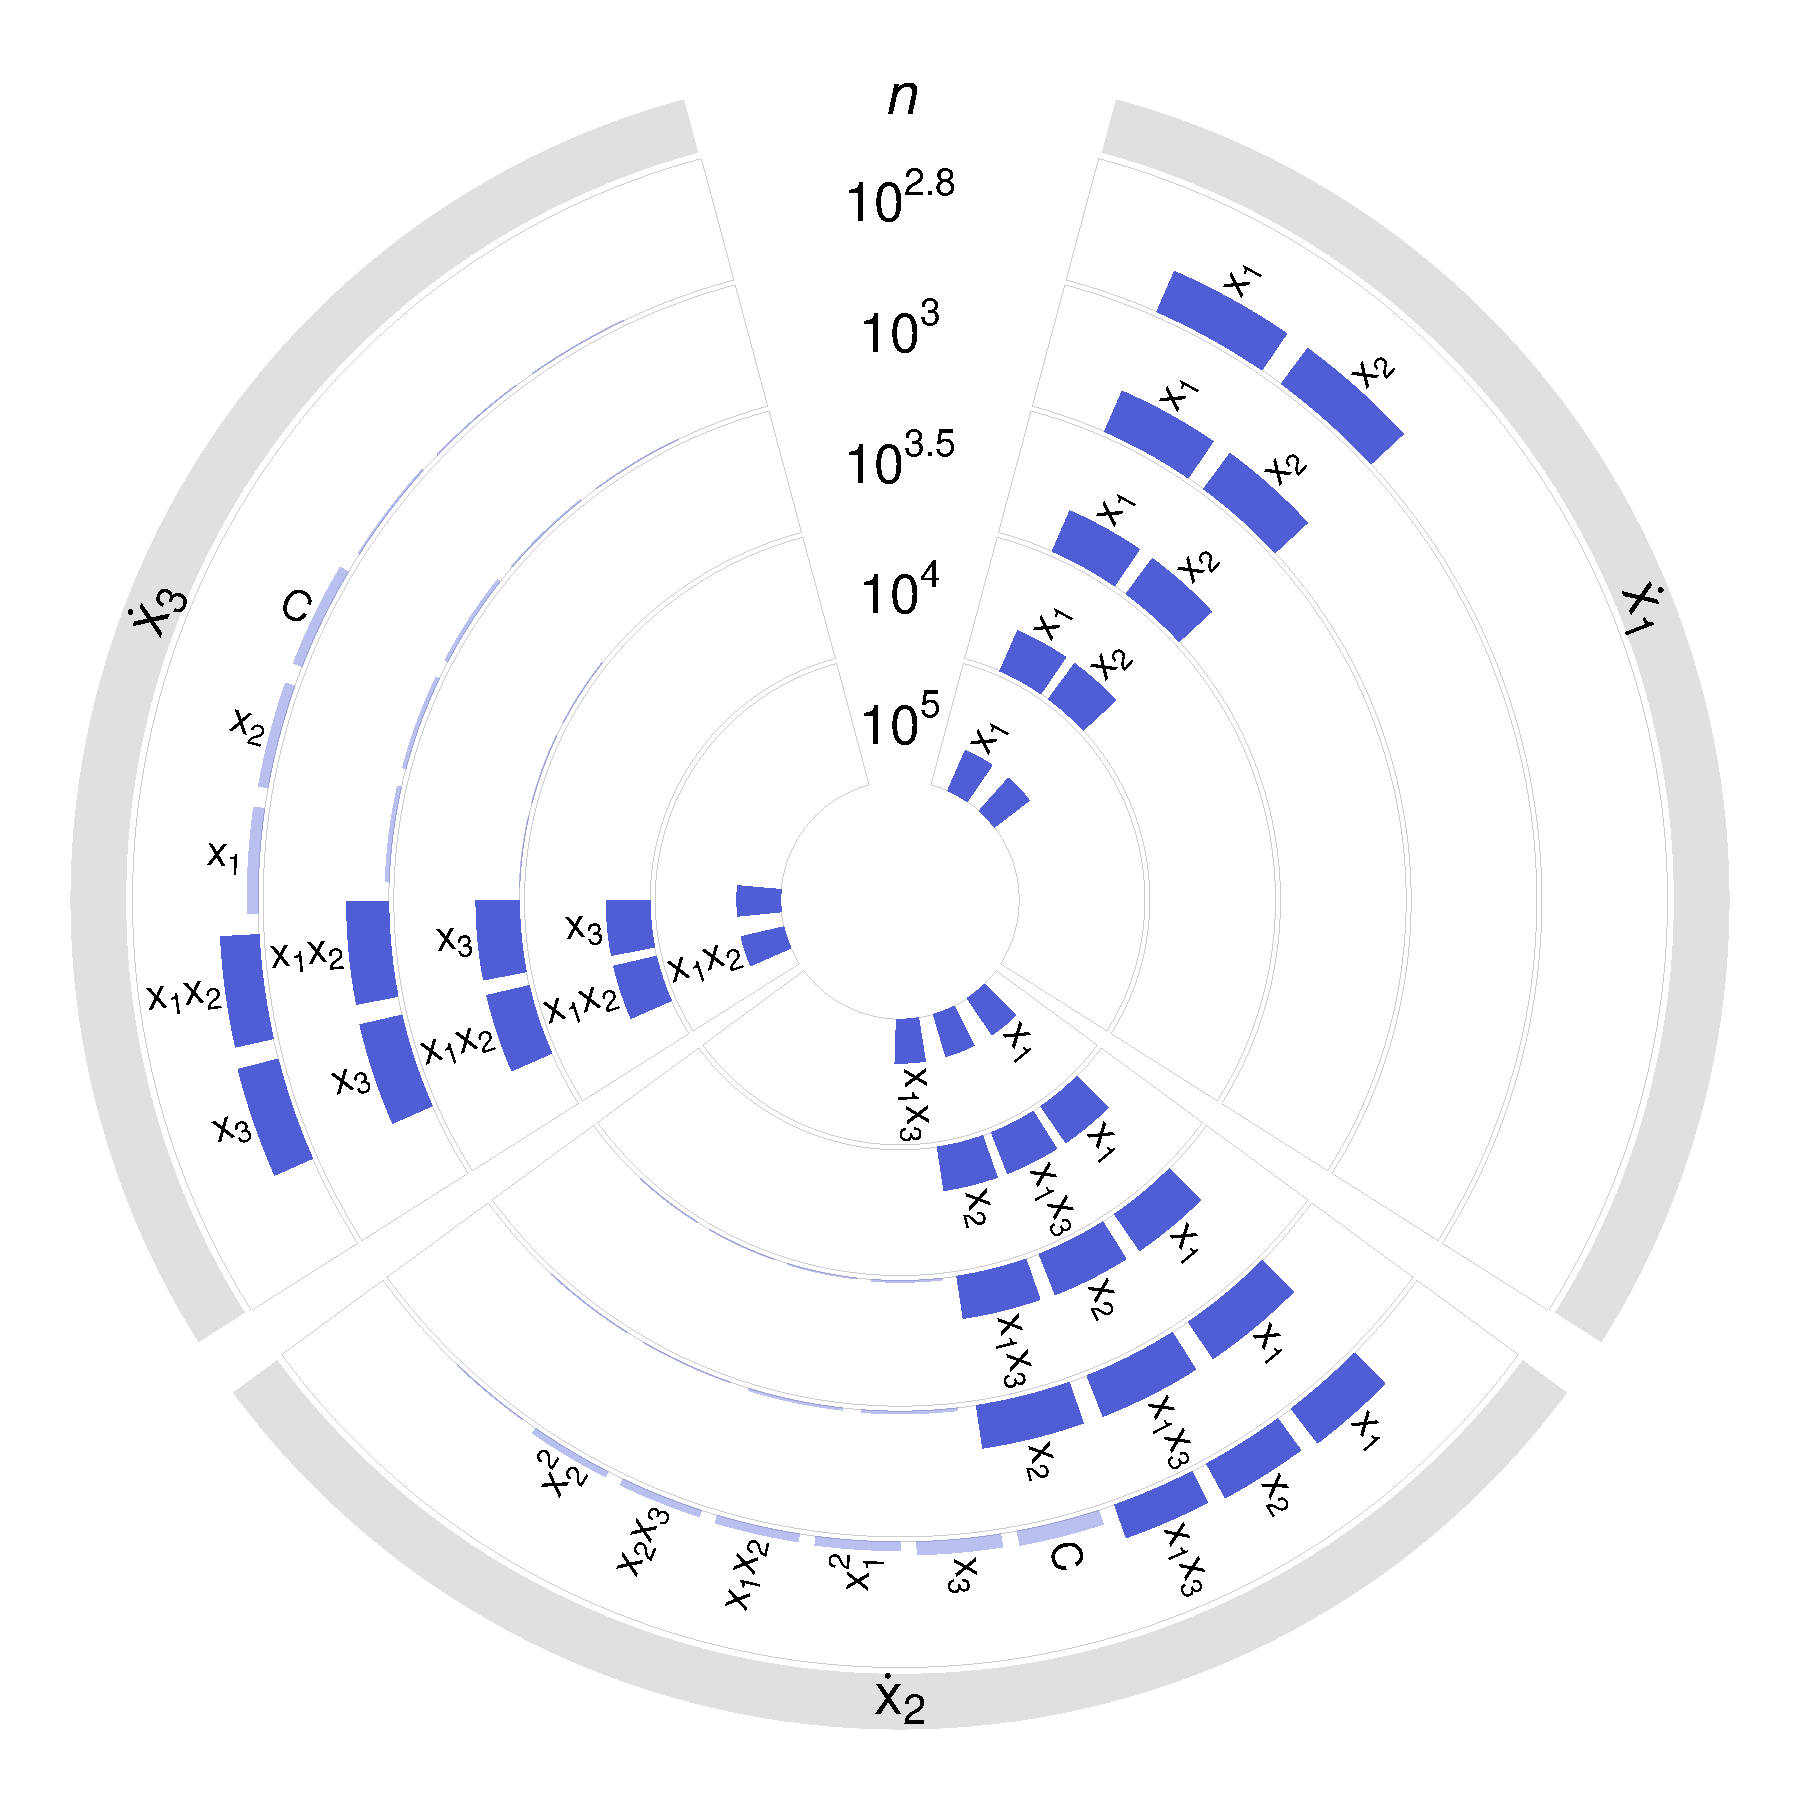
\includegraphics[width=59.000mm]{circ_lorenz_n_ba.pdf}};
\node[anchor=north west, inner sep=0pt] at (62.000,115.456) {\Tag{h}};
\node[anchor=north, inner sep=0pt] at (91.500,115.856) {\Lab{ARGOS}};
\node[anchor=north west, inner sep=0pt] at (62.000,119.456) {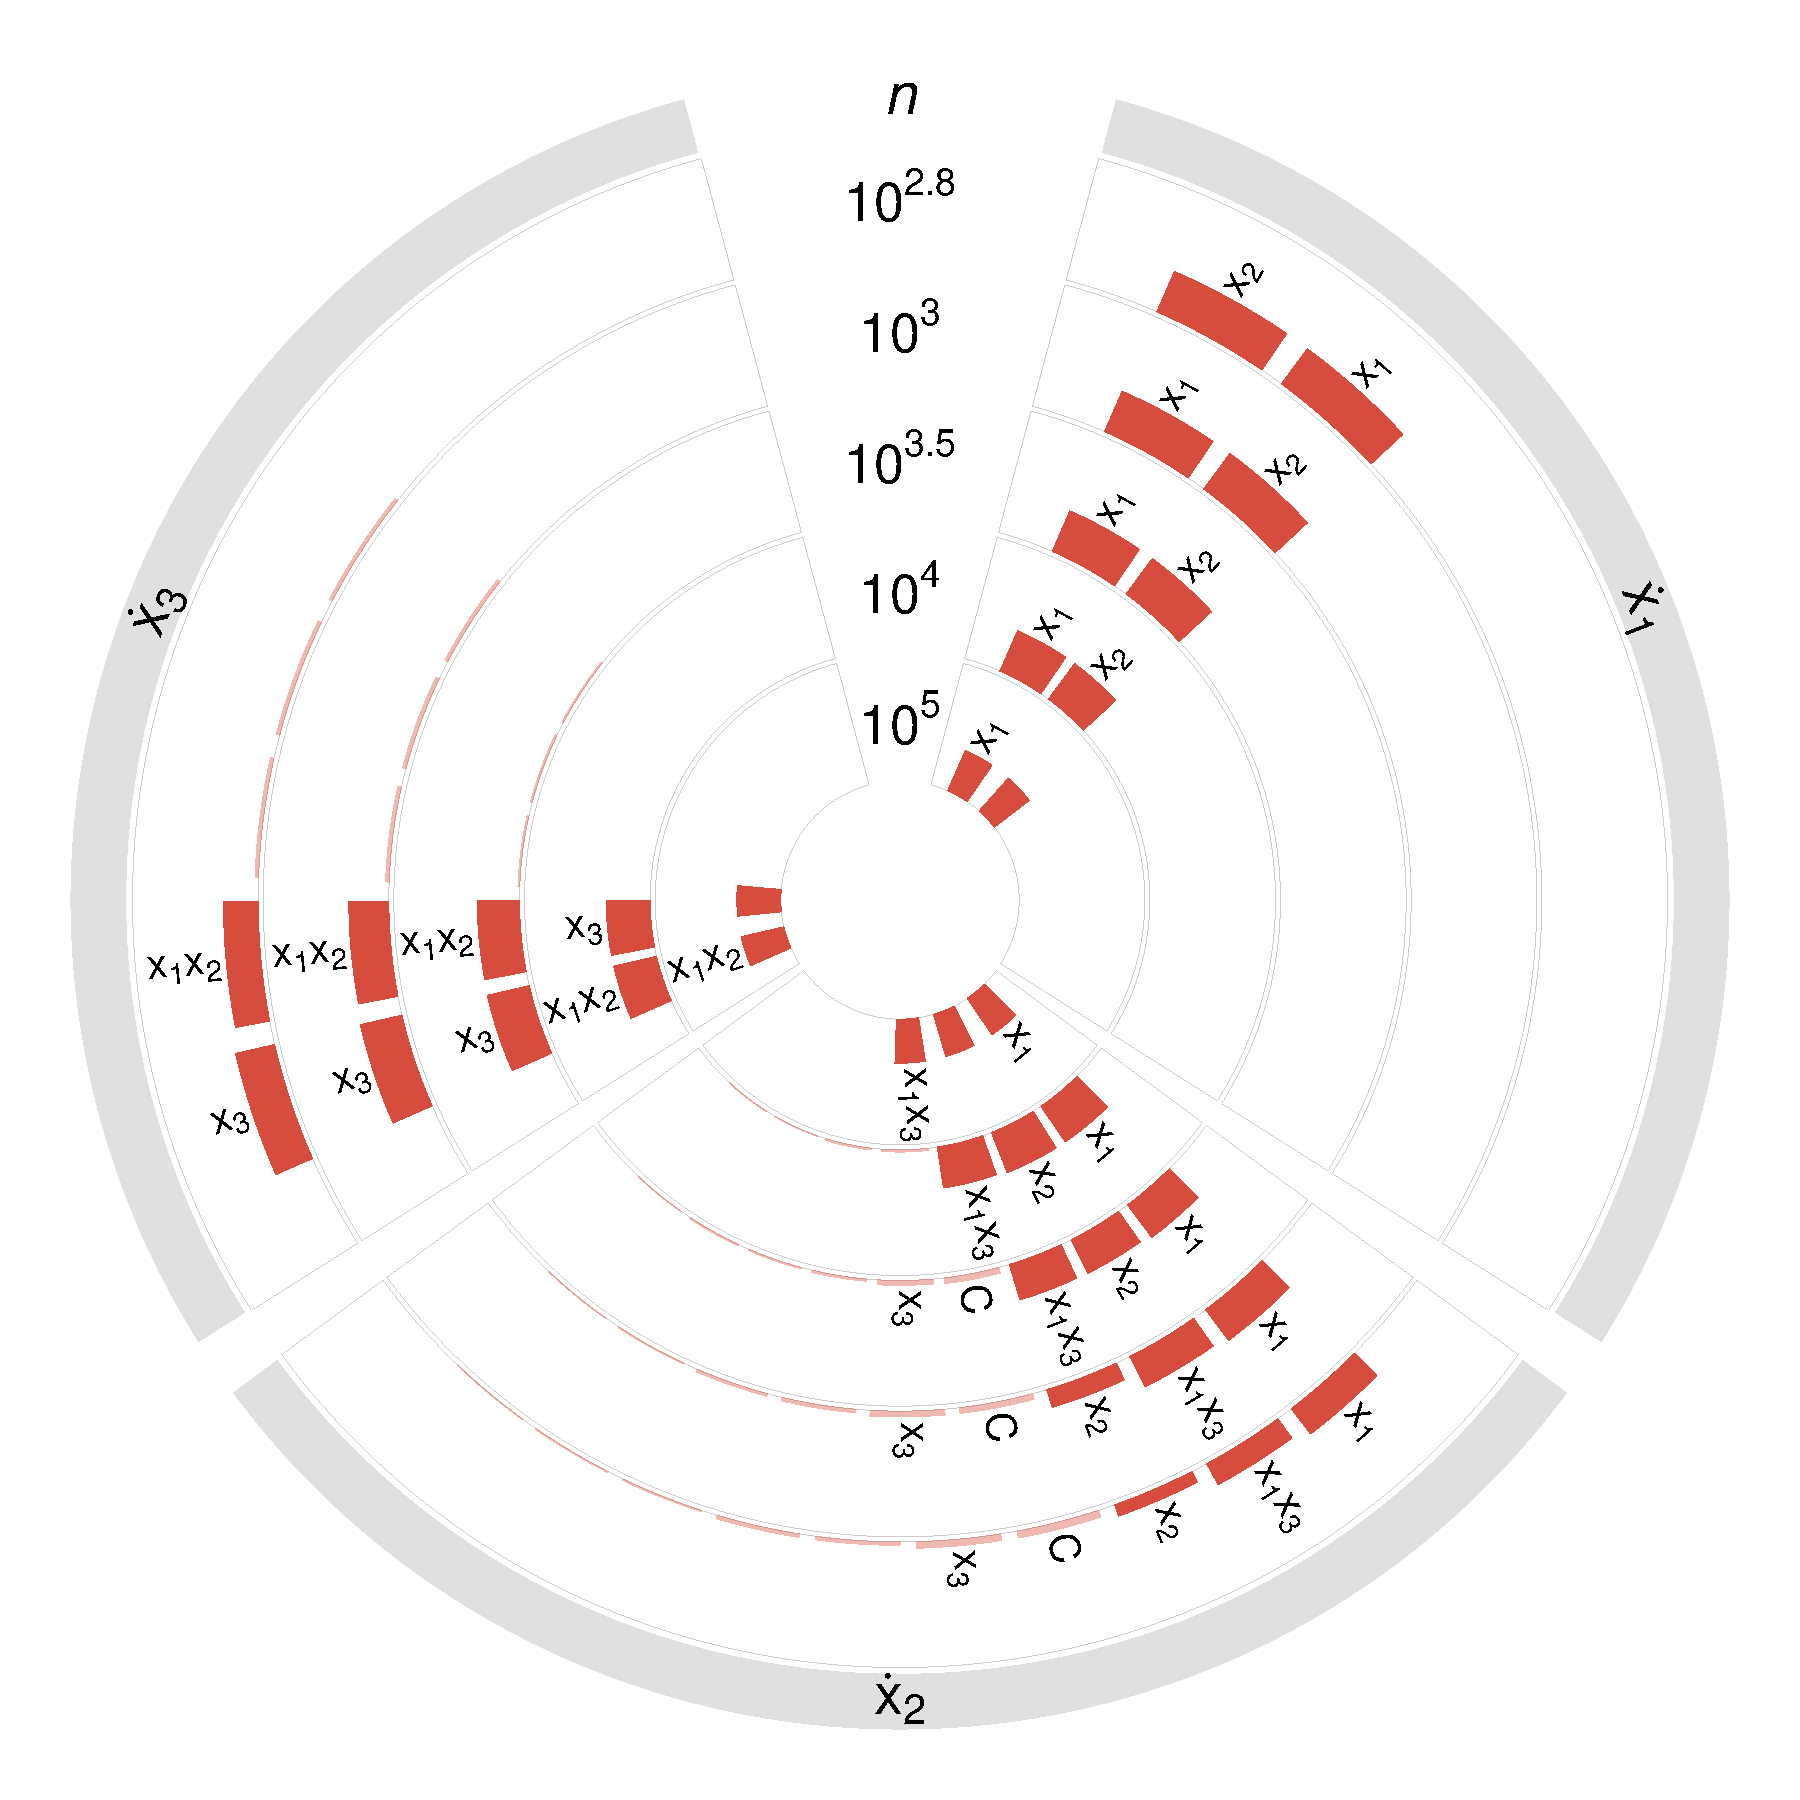
\includegraphics[width=59.000mm]{circ_lorenz_n_argos.pdf}};
\node[anchor=north west, inner sep=0pt] at (124.000,115.456) {\Tag{i}};
\node[anchor=north, inner sep=0pt] at (153.500,115.856) {\Lab{SINDy}};
\node[anchor=north west, inner sep=0pt] at (124.000,119.456) {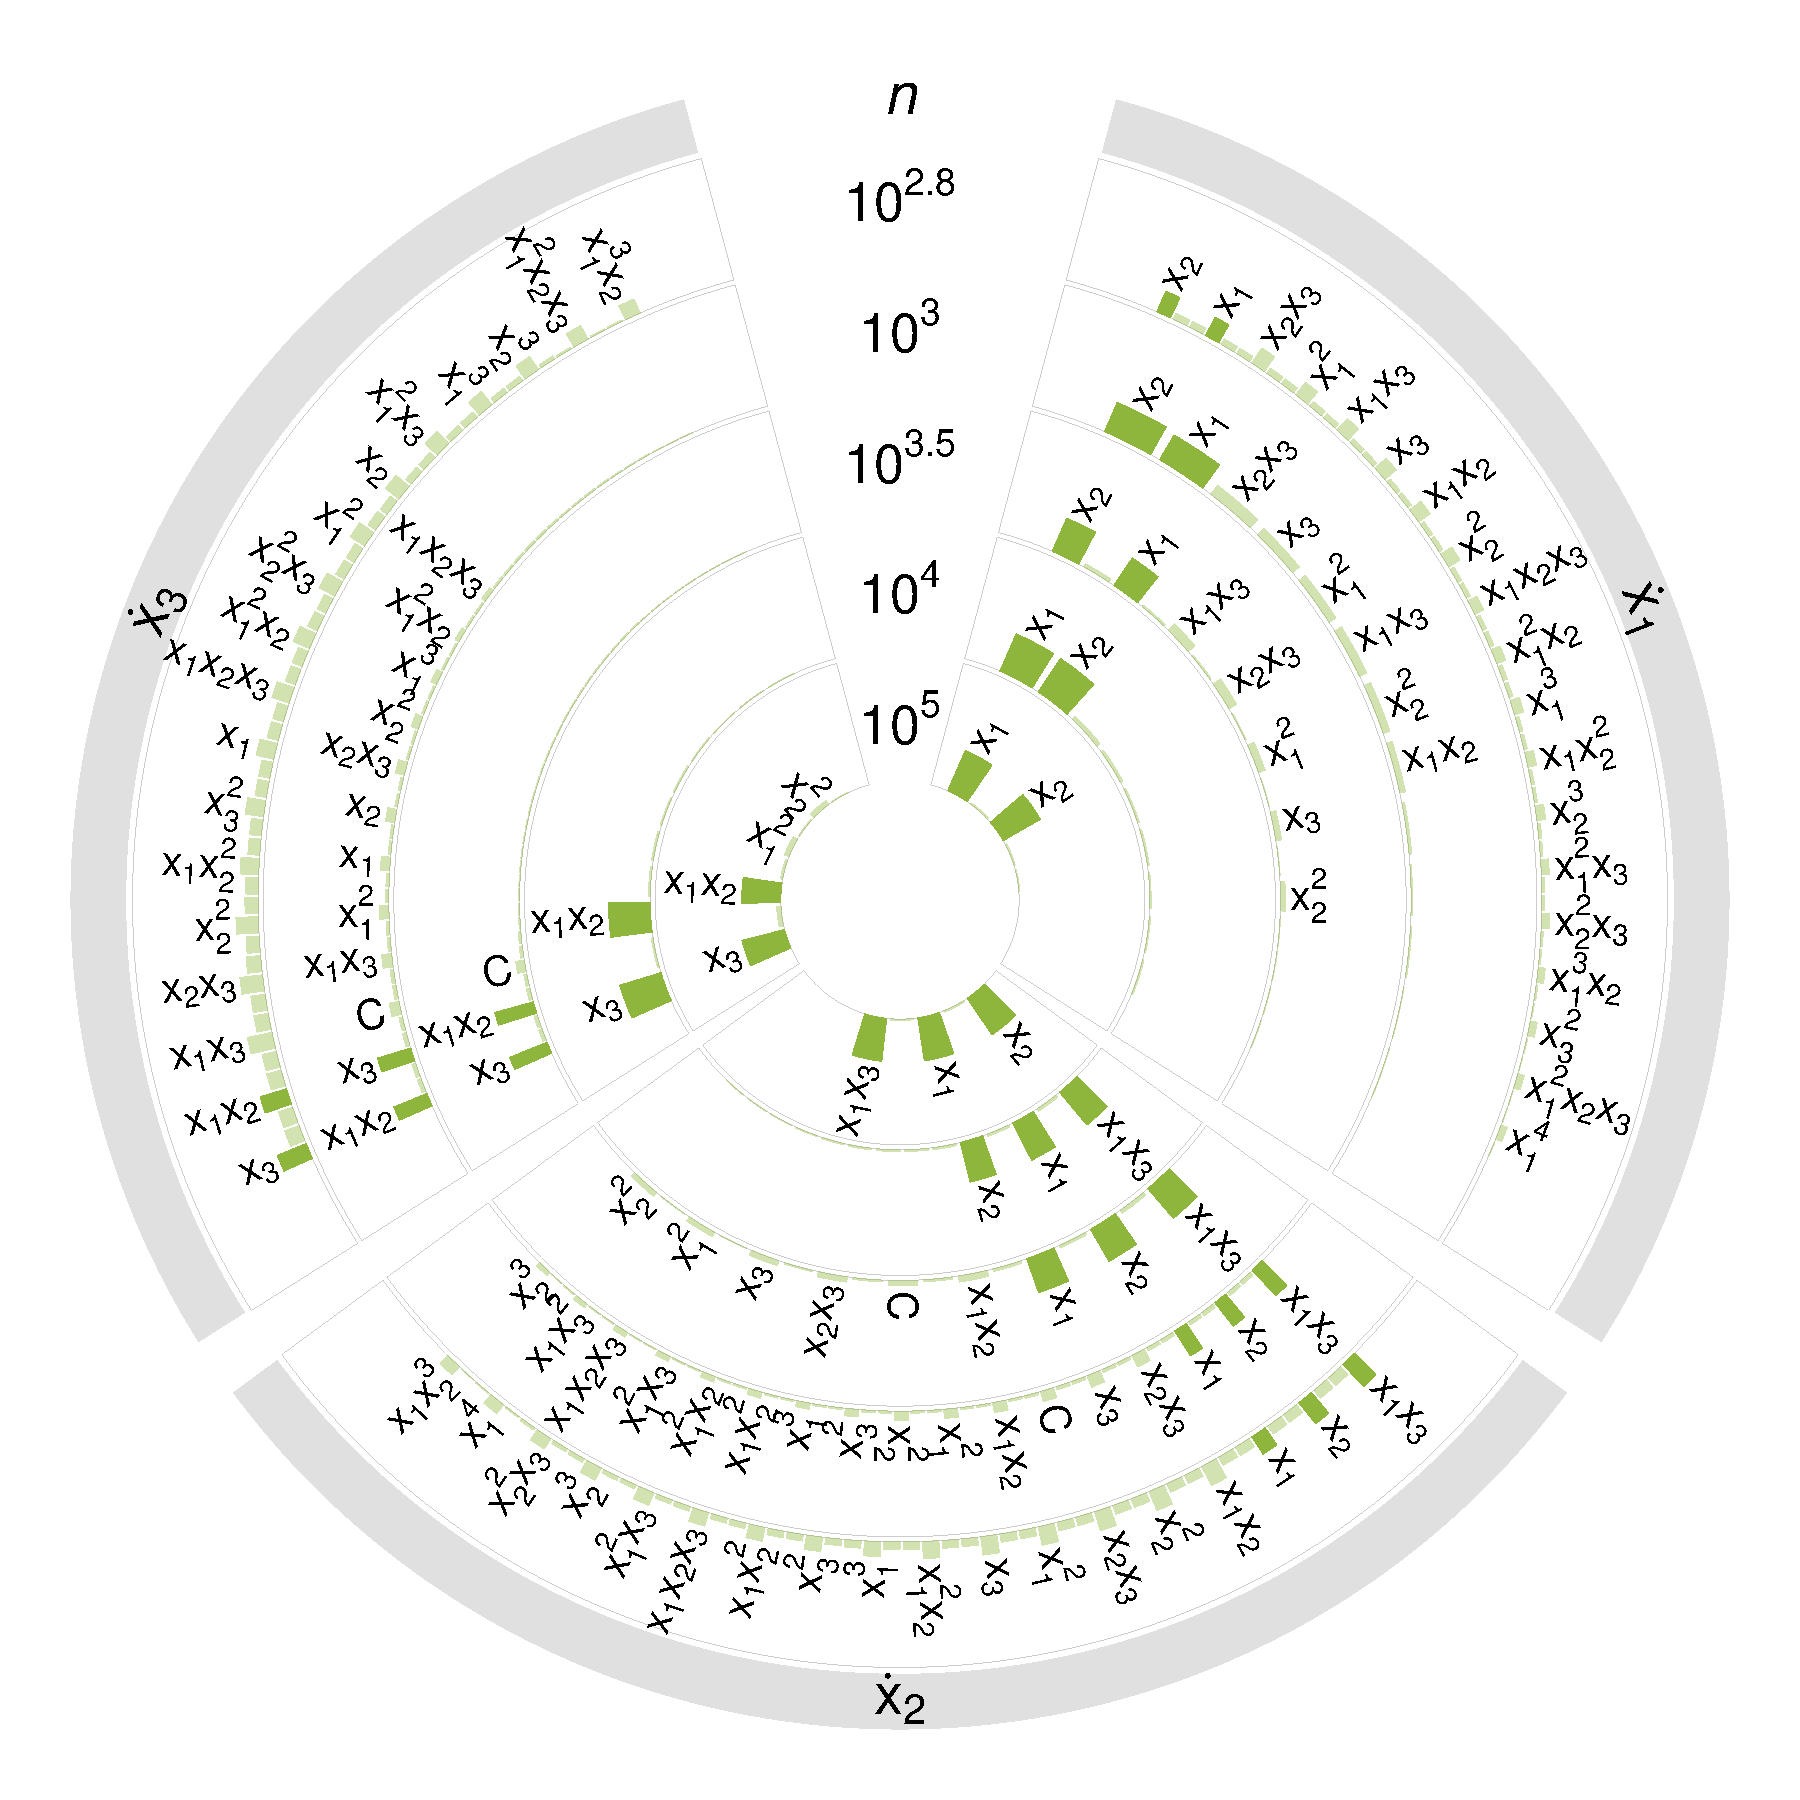
\includegraphics[width=59.000mm]{circ_lorenz_n_sindy.pdf}};
\fill[ba] (31.000,180.456) rectangle ++(2.000,2.000);
\fill[argos] (33.400,180.456) rectangle ++(2.000,2.000);
\fill[sindy] (35.800,180.456) rectangle ++(2.000,2.000);
\node[anchor=west, inner sep=0pt] at (39.000,181.456) {\Lab{true terms}};
\fill[ba!40] (53.000,180.456) rectangle ++(2.000,2.000);
\fill[argos!40] (55.400,180.456) rectangle ++(2.000,2.000);
\fill[sindy!40] (57.800,180.456) rectangle ++(2.000,2.000);
\node[anchor=west, inner sep=0pt] at (61.000,181.456) {\Lab{spurious terms}};
\node[anchor=west, inner sep=0pt] at (82.000,181.456) {\Lab{bar height: selection frequency over 100 trials}};
\end{tikzpicture}
\end{document}
